\chapter*{ЗАКЛЮЧЕНИЕ}
\addcontentsline{toc}{chapter}{\textbf{ЗАКЛЮЧЕНИЕ}}

Распознавание эмоций по звучащей речи -- алгоритмически сложная задача, включающая в себя ряд подзадач, классификация которых была проведена в представленной работе.

На рис. \ref{fig:classification} приведены основные признаки, по которым можно классифицировать системы распознавания.

\begin{figure}[H]
	\centering
	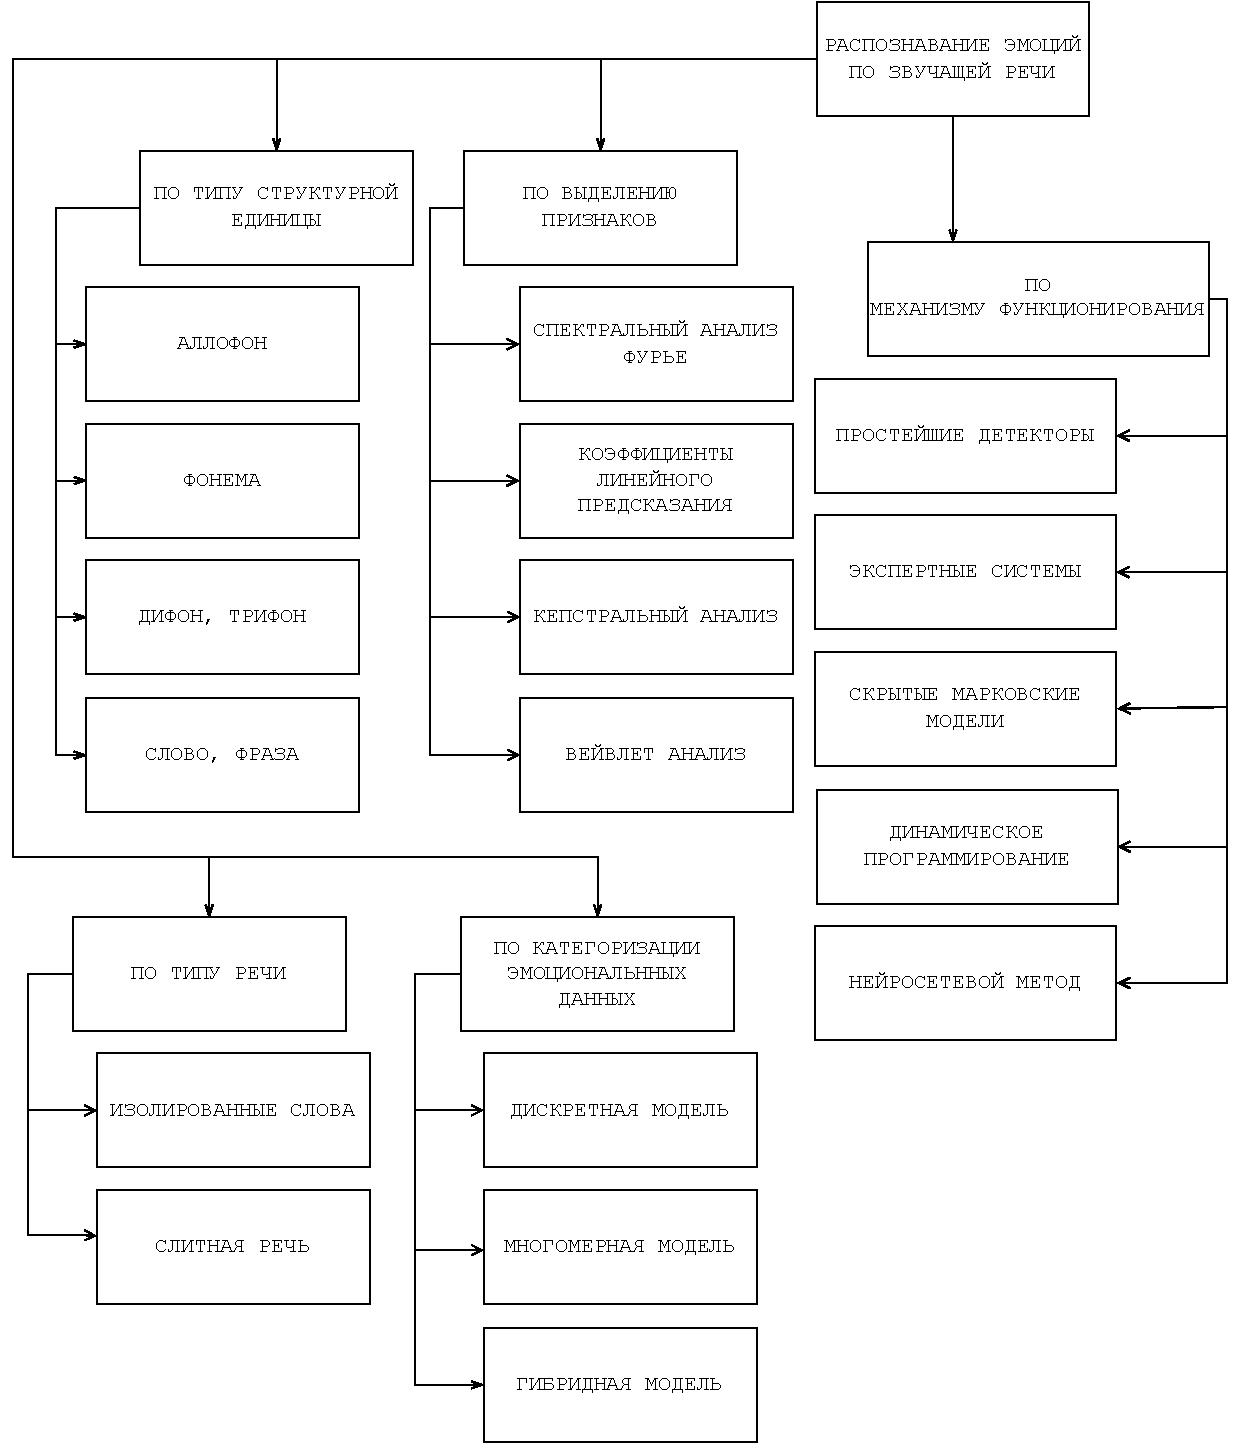
\includegraphics[width=0.85\linewidth]{assets/class}
	\caption{Классификация систем распознавания речи}
	\label{fig:classification}
\end{figure}


Предложена структура системы распознавания эмоций по звучащей речи. 
\begin{enumerate}
	\item Проводится предобработка поступившего на вход аудиофайла.
	\item Извлекаются значимые признаки речевого сигнала.
	\item Проводится предобработка извлеченных признаков. 
	\item Классификатор принимает решение о виде эмоции на основе полученного вектора признаков.
\end{enumerate}

На точность работы систем распознавания оказывает влияние множество факторов. Прежде всего, влияние окружающей среды, а также изменение условий записи.

Корпуса, которые используются для экспериментальной оценки, не всегда способны смоделировать перечисленные ситуации. Поэтому результат существенно зависит от того, насколько представительна база. Результат также зависит от продолжительности материала, используемого в каждом тесте и для создания моделей, и от количества пользователей в корпусе.